\documentclass[12pt]{article}
\usepackage{sbc-template}
\usepackage{graphicx,url}
\usepackage[utf8]{inputenc}
\usepackage[brazilian]{babel}
\usepackage{float}
\usepackage{array}
\usepackage{amsmath,amssymb}

\sloppy

\title{Predição de criminalidade contra pessoas trans e travestis: \\ Relação entre notificações de violência e indicadores municipais no Brasil}

\author{Ana Queiroz da Silva, Natália Metolina, Pedro Henrique Teixeira Soares}

\address{Escola de Artes, Ciências e Humanidades -- Universidade de São Paulo (USP)\\
Rua Arlindo Bétio nº 1000 -- São Paulo -- SP -- Brasil}

  
\begin{document}

\maketitle
     
\begin{resumo}
A violência contra pessoas trans e travestis no Brasil tem pouca visibilidade nas bases oficiais, que raramente separam essa população do conjunto LGBT. Este trabalho usa as denúncias do Disque 100 de 2011 a 2022 (27.441 registros de vítimas LGBT em 2.070 municípios), combinadas a indicadores do IBGE, da pesquisa MUNIC, do Atlas da Violência e do SUS, para identificar os municípios com números alarmantes e prever onde tendem a surgir ondas de denúncias. Depois de unificar os três formatos de registro da base e descontar o porte de cada cidade, 141 municípios tiveram números alarmantes em 2020--2022, 83 deles com menos de 100 mil habitantes. Na previsão de um ano à frente, o LightGBM reduziu o erro em 16,7\% (IC 95\%: 13,3--20,3) em relação a distribuir as denúncias apenas pela população e, monitorando 1\% dos municípios, concentrou 31\% das ondas, contra 22\% da referência. As denúncias foram mais frequentes onde há mais casais do mesmo sexo, maior densidade demográfica e ouvidoria municipal de direitos humanos, e as ondas permaneceram locais, sem se espalhar para cidades vizinhas. As vítimas trans foram 18\% das denúncias com identidade registrada e sofreram violência mais grave e mais pública: em violações contra a vida, a chance de a vítima ser trans foi três vezes maior. Não foi possível medir efeito da criminalização da transfobia pelo STF em 2019: a queda nas denúncias trans começou meses antes e acompanha mudanças no registro, que pesaram mais nos números do que o marco legal.

\textbf{palavras-chave:} violência contra população trans; pessoas trans e travestis no Brasil; Disque 100; previsão espaço-temporal; aprendizado de máquina.
\end{resumo}


\section{Introdução}

A produção de dados referentes à população trans no Brasil é um desafio persistente e uma limitação para a elaboração de políticas públicas. Os Censos elaborados pelo Intituto de Geografia e Estatística (IBGE) não apresentam dados especializados referentes à identidade de gênero. A população transgênera é definida como o conjunto de pessoas que se identificam com um gênero incongruente ou diferente daquele que lhes foi atribuído ao nascer e estima-se que representam entre 0.1\% a 2\% da população brasileira, a depender da localidade. Estima-se que o total da população transgênera no Brasil se distribua da seguinte forma: Norte 8\%, Nordeste 26\%, Centro-Oeste 7\%, Sudeste 44\% e Sul 15\ \cite{spizziri_eufrasio_lima:2021}. Travestis  são uma identidade de gênero revindicada na América Latina, reunindo pessoas designadas como do sexo masculino ao nascer, mas que se identificam com o feminino, embora não necessariamente se identifiquem como mulheres \cite{leal_silva_lizzi:2026}. Para fins de pesquisa abarcaremos as categorias "transgênero", "travesti" e "transexual", esta última presente em bases de dados e documentos oficiais dos programas de saúde públicos, atendendo as diversas fontes utilizadas no trabalho.

A violência é um fenômeno complexo e polissêmico, sendo delimitado neste trabalho às definições presentes na Classificação Internacional de Doenças, caracterizando-se pelo uso intencional da força ou poder que possa ocasionar lesão, morte, privação, deficiência ou dano psicológico \cite{marinho_tomazelli_firianelli:2024}. Em 2011 a notificação de violência autoprovocada e interpessoal integrou a lista de notificação compulsória e foi incluída no Sistema de Informação de Agravos de Notificação (Sinan) e em 2014, para contemplar a Política Nacional de Saúde Integral de Lésbicas, Gays, Bissexuais, Travestis e Transexuais, foram incluídas na ficha de notificação as variáveis “orientação sexual”, “identidade de gênero” e "nome social". Em 2019, o Supremo Tribunal Federal (STF) incluiu a transfobia nos crimes previstos na Lei do Racismo (Lei nº 7.716/1989). Dados produzidos e organizados por associações e ONGs nacionais e internacionais indicam o Brasil como líder nos índices de violência e mortalidade por crimes violentos decorrentes da transfobia. O Sinan e o DATASUS tornaram-se as principais fontes de dados para as análises acadêmicas. Uma fonte menos explorada é o Disque Direitos Humanos (Disque 100), que recebe, por telefone e outros canais, denúncias de violações de direitos humanos feitas pela própria vítima ou por terceiros, e que mantém desde 2011 um recorte específico para a população LGBT. Diferente do Sinan, que registra os casos que chegam a um serviço de saúde, o Disque 100 também capta violências que raramente geram atendimento, como a discriminação e a violência psicológica. Todas essas bases, no entanto, enfrentam um cenário de subnotificação e dificuldade de desagregação da população trans do conjunto da população LGBT+, não representando com fidelidade a realidade da violência contra trans e travestis no Brasil.

As políticas nacionais de saúde voltadas especificamente para a população trans, que exercem um papel fundamental no acolhimento institucional, começaram a ser estruturadas e ampliadas de forma mais consistente nas últimas décadas, tendo como marcos fundamentais o Processo Transexualizador, formalizado em 2008, a Política Nacional de Saúde Integral LGBT, instituída em 2011, e a portaria do Ministério da Saúde de 2009, que assegura o direito ao uso do nome social em atendimentos prestados na rede pública de saúde, conquista esta que posteriormente foi convertida em decreto federal no ano de 2016. O Processo Transexualizador, no entanto, ainda é um programa com pouca distribuição pelo território nacional, tendo atualmente 26 municípios no país, em sua maioria grandes centros urbanos, concentrando-se principalmente nas regiões Sudeste e Sul, seguidos do Nordeste.

A partir deste cenário, o trabalho parte da constatação de que crimes contra a população LGBT, e em especial contra pessoas trans e travestis, têm pouca visibilidade, e de que saber onde as denúncias são desproporcionalmente altas é um primeiro passo para direcionar essa atenção. O objetivo é identificar os municípios brasileiros com números alarmantes de denúncias de violência contra pessoas LGBT e, a partir das suas tendências e características, prever em quais cidades tendem a surgir ondas de denúncias. Como a amostra de vítimas trans é pequena, as análises sempre comparam esse grupo com o total da comunidade LGBT. Quatro perguntas guiam o trabalho: (i) onde estão e como se agrupam os municípios com números alarmantes; (ii) se indicadores municipais permitem prever ondas de denúncias e qual modelo o faz melhor; (iii) em que a violência contra pessoas trans difere da violência contra as demais pessoas LGBT, em proporção e em perfil; e (iv) se a inclusão da transfobia na Lei do Racismo pelo STF, em 2019, alterou o número de denúncias. Os fatores associados a mais denúncias mostram onde o registro funciona e onde ele falta. O reforço desses fatores pode ampliar a notificação da violência e, como consequência, tornar as bases de dados mais consistentes para a elaboração de políticas de prevenção de crimes que vitimam a população trans.


\section{Trabalhos Correlatos}

Os estudos a respeito da violência contra a população trans no Brasil concentram-se em estudos ecológicos observacionais com análise espaço-temporal por modelos lineares generalizados (2015-2023) \cite{leal_silva_lizzi:2026} e epidemiológicos (2015-2022) através de regressão linear generalizada baseada em notificações disponibilizados pelo Sistema de Informação de Agravos de Notificação (Sinan) \cite{marinho_tomazelli_firianelli:2024}. O pareamento entre notificações de violência contra pessoas transgêneras e a mortalidade desta população por causas violentas (2014-2022) apresentou um importante panorama referente à reincidência de crimes e à violência autoprovocada, identificando fatores de risco \cite{luis:2025}. O estudo transversal de Luis et al. (2024) apresenta um ganho de consistência nos resultados ao normalizar as bases de dados do Sistema de Informação de Agravos de Notificação (Sinan) e do Sistema de Informações sobre Mortalidade (SIM) através da identificação de nomes das vítimas obtidos por meio de solicitação à Secretaria de Vigilância em Saúde e Ambiente, com assinatura dos autores do estudo do registro de responsabilidade e confidencialidade. 

Os trabalhos citados indicam a mesma conclusão geral: as notificações ainda não representam a realidade da violência contra transgêneros no Brasil devido à subnotificação e à dificuldade de desagregação da população trans do conjunto dos dados sobre a população LGBT+ disponibilizados na bases institucionais. O crescimento do número de municípios com notificações, no entanto, indicam um aumento da visibilidade e enfrentamento à violência contra este recorte da população. Aproximando os resultados dos três estudos, as notificações de violência contra a população trans corresponde aproximadamente a 1.4\% do total de notificações no Sinan. Em relação às notificações contra a população trans, a concentração de vítimas foi de mulheres (65,3\%), jovens entre 19 e 29 anos (36,1\%) e negras. % [completar com o percentual de vítimas negras da referência]

Fora do recorte trans, trabalhos recentes aplicaram aprendizado de máquina a notificações de violência contra a mulher, combinando o Sinan com dados do IBGE para projetar tendências e classificar tipos de violência com florestas aleatórias e LightGBM (Tabela~\ref{tab:referencia}). Esses estudos mostram que algoritmos baseados em árvores de decisão conseguem extrair padrões de bases administrativas de violência, mas não foram aplicados à população LGBT nem avaliados quanto à capacidade de antecipar onde os casos vão se concentrar.

Este trabalho se diferencia da literatura em quatro pontos. Primeiro, usa o Disque 100 em vez do Sinan, o que permite observar violências que não chegam ao serviço de saúde: a violência psicológica e a discriminação, que estão na maioria das denúncias, raramente geram uma notificação no Sinan. Segundo, cobre todos os 5.565 municípios e combina as denúncias com indicadores municipais, entre eles a proporção de domicílios com casais do mesmo sexo do Censo 2022, a melhor aproximação disponível do tamanho da população LGBT visível em cada cidade. Terceiro, além de explicar, \textit{prevê}: os modelos são avaliados prevendo anos que não viram, como aconteceria no uso real, e comparados com regras simples. Quarto, trata explicitamente as mudanças no sistema de registro do Disque 100, que, como mostram os resultados, pesam mais nos números do que os marcos legais.

\begin{table}[H]
\centering
\caption{Comparativo entre abordagens da literatura e este trabalho}
{\renewcommand{\arraystretch}{1.5}

\begin{tabular}{>{\raggedright\arraybackslash}p{3.2cm} >{\raggedright\arraybackslash}p{3.2cm} >{\raggedright\arraybackslash}p{3.2cm} >{\raggedright\arraybackslash}p{3.2cm}}
\hline
\textbf{Referência} & \textbf{Método} & \textbf{Dados utilizados} & \textbf{Objetivo}\\
\hline
Leal, G.C. et al. (2026) & Modelagem Bayesiana Hierárquica (regressão de Poisson) e Aproximações de Laplace Aninhadas Integradas (INLA) & Sinan & Análise espaço-temporal das notificações de violência contra a população trans entre 2015 e 2023
\\
Luis, M.A. et al. (2024) & Modelo de Poisson & Sinan e SIM & Identificar os fatores associados à mortalidade de pessoas trans por causas violentas entre 2014 e 2022
\\
Marinho, K.R.E. et al. (2024) & Estudo epidemiológico e método de Prais-Winsten & Sinan & Análise da tendência temporal e características das notificações de violência contra a população trans entre 2015 e 2022
\\
Coelho, M.M.F. et al. (2025) & Prophet e Random Forest & Sinan e IBGE & Análise temporal e projeção da violência contra a mulher de 2013 a 2033
\\
Lucca, R. e Romero, R. (2026) & Random Forest e LightGBM & Sinan & Analisar tipos de violência contra a mulher entre 2018 e 2024
\\
\hline
\textbf{Este trabalho} & Bayes empírico, Getis-Ord, modelo endêmico-epidêmico, LightGBM, Extra Trees e série temporal interrompida & Disque 100, IBGE, MUNIC, Atlas da Violência e SUS & Identificar municípios com números alarmantes e prever ondas de denúncias de violência contra pessoas LGBT e trans entre 2011 e 2022
\\
\hline
\end{tabular}
}
\label{tab:referencia}
\end{table}


\section{Método}

Este é um estudo ecológico: ele analisa municípios, e não pessoas. Para cada um dos 5.565 municípios brasileiros e cada ano de 2011 a 2022, reunimos o número de denúncias de violência contra pessoas LGBT e um conjunto de características do município. O trabalho tem quatro análises, cada uma com seu código, e todas respondem à mesma pergunta central: \textbf{onde a violência notificada é alarmante e quais cidades tendem a ter ondas de notificações}.

\subsection{Coleta de dados}

\textbf{Denúncias.} A fonte das notificações é o Disque Direitos Humanos (Disque 100), mantido pela Ouvidoria Nacional de Direitos Humanos do Ministério dos Direitos Humanos e da Cidadania. Usamos as denúncias cadastradas entre janeiro de 2011 e dezembro de 2022 em que a vítima pertence ao grupo ``população LGBTQIA+'', o que deu 50.045 linhas. De cada denúncia aproveitamos quatro tipos de informação: quando e onde ocorreu (data e município da vítima); quem é a vítima (gênero, identidade de gênero, orientação sexual, idade e raça/cor); o que aconteceu (tipo de violação, local e relação com o agressor); e como foi denunciado (quem denunciou e por qual canal, informação que só existe a partir de 2020).

\textbf{Características dos municípios.} Os dados municipais vieram de fontes oficiais e foram baixados por um script, o que torna a coleta reproduzível (Tabela~\ref{tab:fontes}). Do IBGE vieram população, área, PIB, renda, composição por cor ou raça e idade, e o número de domicílios com casal do mesmo sexo. Também do IBGE, a pesquisa MUNIC informa se a prefeitura tem órgão, conselho, programa ou ouvidoria de direitos humanos e políticas para a população LGBT. Do Atlas da Violência (Ipea) veio o número de homicídios, e do Atlas do Desenvolvimento Humano, o IDHM e o índice de Gini. A presença do Processo Transexualizador foi medida pelo número de procedimentos registrados por ano no SUS (SIA/SIH) nos 26 municípios habilitados. Por fim, a localização de cada município (o ponto central do seu território) foi usada para definir quais são as cidades vizinhas.

Nem todas as fontes tiveram o mesmo peso nos resultados (última coluna da Tabela~\ref{tab:fontes}). O próprio Disque 100 é a base mais importante: além de fornecer as denúncias, o histórico de cada município foi a informação que mais contribuiu para a previsão. Entre os indicadores municipais, três vieram do IBGE e concentraram o poder explicativo: a proporção de domicílios com casal do mesmo sexo, que mede a população LGBT visível de cada cidade, a densidade demográfica e a composição por cor ou raça. Da MUNIC, a variável relevante foi a existência de ouvidoria de direitos humanos. Renda, PIB, desigualdade, homicídios e Processo Transexualizador foram testados e não mostraram relação com o volume de denúncias, o que também é um resultado.

\begin{table}[H]
\centering
\caption{Fontes de dados, variáveis municipais e seu papel nos resultados}
\label{tab:fontes}
{\renewcommand{\arraystretch}{1.3}\small
\begin{tabular}{>{\raggedright\arraybackslash}p{4.2cm} >{\raggedright\arraybackslash}p{3.8cm} >{\raggedright\arraybackslash}p{1.9cm} >{\raggedright\arraybackslash}p{3.4cm}}
\hline
\textbf{Variável} & \textbf{Fonte} & \textbf{Período} & \textbf{Papel nos resultados} \\
\hline
Denúncias de violência contra pessoas LGBT & Disque 100 (ONDH/MDHC) & 2011--2022 & variável prevista; o histórico é o principal preditor \\
Domicílios com casal do mesmo sexo & IBGE, Censo 2022 & 2022 & fator mais forte (mais denúncias) \\
Área e densidade demográfica & IBGE, Censo 2022 & 2022 & forte (mais denúncias) \\
População residente & IBGE (estimativas anuais e Censo 2022) & 2011--2022 & base do valor esperado \\
Cor ou raça; população de 15 a 29 anos & IBGE, Censos 2010 e 2022 & 2010, 2022 & pretos e pardos: menos denúncias; jovens: sem efeito \\
Políticas municipais de direitos humanos e LGBT & IBGE, MUNIC & 2014, 2019, 2023 & ouvidoria: mais denúncias; índice LGBT: sem efeito no total \\
PIB municipal & IBGE, PIB dos Municípios & 2011--2022 & sem efeito \\
Renda domiciliar por pessoa & IBGE, Censos 2010 e 2022 & 2010, 2022 & sem efeito \\
Homicídios registrados & Ipea/FBSP, Atlas da Violência & 2011--2022 & sem efeito \\
IDHM e índice de Gini & Atlas do Desenvolvimento Humano & 2010 & Gini: sem efeito; IDHM fora dos modelos \\
Procedimentos do Processo Transexualizador & SUS (SIA/SIH) & 2008--2026 & sem efeito \\
\hline
\end{tabular}}
\end{table}

\subsection{Limpeza e Normalização dos Dados}

A base do Disque 100 não é uma tabela única e homogênea. Ao longo do período, o sistema de registro mudou três vezes: de 2011 a 2019, no primeiro semestre de 2020 e de julho de 2020 em diante. A cada mudança, as colunas trocaram de nome, as categorias de resposta mudaram e até o significado de uma linha mudou. No formato mais recente, cada linha deixou de ser uma denúncia e passou a ser uma violação, de modo que a mesma denúncia aparece várias vezes. O tratamento teve cinco objetivos.

\textbf{1. Contar cada caso uma vez.} Removemos 561 linhas repetidas e agrupamos as linhas que pertenciam à mesma denúncia e à mesma vítima. A base final tem 27.441 registros, cada um correspondendo a uma vítima em uma denúncia.

\textbf{2. Falar a mesma língua em todos os anos.} Padronizamos a escrita (maiúsculas, sem acentos) e unificamos as colunas equivalentes dos três formatos. Respostas como ``não informado'' ou ``não sabe'' foram reunidas na categoria ``desconhecido'', em vez de descartar o registro. As cerca de 240 descrições diferentes de violação foram agrupadas em nove tipos: contra a vida, sexual, institucional, discriminação, patrimonial, negligência, contra a liberdade, física e psicológica. Uma denúncia pode ter mais de um tipo.

\textbf{3. Identificar as vítimas trans.} A informação de que a vítima é travesti, transexual ou transgênero foi registrada em campos diferentes ao longo do tempo. Entre julho de 2020 e junho de 2022, o formulário simplesmente não tinha essa opção. Nesse intervalo, tratamos a informação como desconhecida, e não como zero, para não concluir erroneamente que não houve vítimas trans.

\textbf{4. Localizar cada caso.} Associamos cada registro ao código oficial do seu município. Isso foi possível em 97,6\% dos casos, que se distribuem por 2.070 municípios.

\textbf{5. Montar o painel de municípios.} Somamos os registros por município e ano. Os municípios sem nenhuma denúncia entram com zero: esse zero também é informação. Seis municípios criados depois de 2010 ficaram de fora por não terem dados em todos os anos. Os valores em dinheiro foram corrigidos pela inflação para reais de 2022. Os dados que só existem nos Censos de 2010 e 2022 foram estimados para os anos intermediários. Das três edições da MUNIC, aproveitamos as sete perguntas presentes em todas e as somamos num índice de política LGBT de 0 a 4. O Processo Transexualizador foi considerado ativo nos anos em que o município realizou ao menos um procedimento: dos 26 municípios com o serviço, só 10 tiveram atividade dentro do período estudado.

Por fim, todas as variáveis foram convertidas em números que os modelos conseguem usar. As categorias viraram colunas de 0 e 1, e as medidas muito desiguais entre municípios (como população e PIB) foram colocadas em escala logarítmica e padronizadas.

\subsection{Análise Estatística das Notificações de Violência e Correlação entre Variáveis}

\textbf{Duas características dos dados guiaram as escolhas.} A primeira é que a grande maioria dos municípios quase não aparece na base: 63\% nunca registraram uma denúncia no período, e em 91\% das combinações de município e ano o número é zero. Contagens assim exigem modelos próprios para dados com muitos zeros e muita variação. A segunda é que o volume nacional de denúncias sobe e desce por razões administrativas do próprio Disque 100, como trocas de sistema e de formulário, e não por mudanças na violência. Por isso, separamos as duas perguntas: \textit{quanto} o país registra num ano (tratado como um dado conhecido) e \textit{onde} esses registros se concentram (o que os modelos tentam explicar e prever). Para cada município e ano calculamos um \textbf{valor esperado}: quantas denúncias o município teria se recebesse uma fatia do total nacional proporcional à sua população. Comparar o observado com esse esperado é a base de todas as análises (fórmula A1 no Apêndice).

\textbf{Análise 1 --- Onde estão os números alarmantes e quais cidades tendem a ter ondas.} Esta é a análise central e tem quatro etapas.

\begin{itemize}
\item \textit{Risco relativo.} Para cada município, dividimos as denúncias observadas pelas esperadas. Um risco relativo de 2 significa o dobro do esperado para o porte da cidade. Em cidades pequenas, porém, uma única denúncia já gera um risco enorme por puro acaso. Para evitar esse falso alarme, usamos a \textbf{suavização bayesiana empírica} \cite{marshall:1991}, que puxa os valores de cidades pequenas em direção à média nacional na medida da sua incerteza (fórmula A2). Consideramos \textbf{alarmante} o município cuja chance de estar acima do esperado passa de 95\%.
\item \textit{Aglomerados regionais.} Para saber se as cidades alarmantes formam regiões, usamos a estatística de \textbf{Getis-Ord} \cite{getis_ord:1992}, que compara cada município e seus 10 vizinhos mais próximos com o restante do país (fórmula A3).
\item \textit{Previsão.} Para prever quantas denúncias cada município terá no ano seguinte, comparamos três modelos. O \textbf{modelo endêmico-epidêmico} \cite{held_hohle_hofmann:2005}, criado para acompanhar surtos de doenças, divide o volume esperado de cada cidade em três partes: o que se explica pelas suas características (parte estrutural), o que se explica pelo próprio histórico (inércia) e o que vem das cidades vizinhas (propagação), conforme a fórmula A4. Ele foi escolhido por permitir interpretar \textit{por que} uma cidade é alarmante. O \textbf{LightGBM} \cite{ke:2017} é um algoritmo de aprendizado de máquina baseado em árvores de decisão, escolhido por costumar ter a maior precisão nesse tipo de dado. O \textbf{Extra Trees} \cite{geurts:2006}, da mesma família das florestas aleatórias usadas na literatura (Tabela~\ref{tab:referencia}), foi incluído para comparação. Os três foram comparados com regras simples: distribuir as denúncias apenas pela população, repetir a fatia histórica de cada cidade e repetir o número do ano anterior.
\item \textit{Alertas de onda.} Definimos \textbf{onda} como um ano em que o município tem pelo menos 5 denúncias e pelo menos o dobro do esperado. Seguindo a lógica dos sistemas de vigilância de surtos \cite{farrington:1996}, um município entra em \textbf{alerta} quando o número observado supera o limite que o modelo considerava plausível em 95\% dos casos (fórmula A5).
\end{itemize}

Para avaliar a previsão de forma honesta, simulamos o uso real: cada modelo aprendeu apenas com os anos anteriores e tentou prever o ano seguinte, como se ainda não o conhecesse, repetindo o processo para cada ano de 2016 a 2022. Medimos o erro de cada modelo, quantas das 50 cidades com mais denúncias ele acertou e, entre as 20 cidades que ele apontou como mais prováveis de ter uma onda, quantas de fato a tiveram. Para verificar como o LightGBM aprende e se o resultado é confiável, registramos o erro a cada árvore adicionada (curvas de aprendizado), reamostramos os municípios 2.000 vezes para obter intervalos de confiança (\textit{bootstrap}), treinamos o modelo com partes das informações para medir a contribuição de cada grupo, variamos seus parâmetros para testar a sensibilidade e calculamos os valores SHAP, que mostram quanto cada informação pesou em cada previsão.

\textbf{Análise 2 --- A violência atinge mais as pessoas trans em certos municípios?} Calculamos, para cada município e ano, a proporção de vítimas trans entre todas as denúncias LGBT, usando só os períodos em que a identidade trans podia ser registrada. Uma \textbf{regressão binomial} (fórmula A6) mostra quais características do município se associam a uma proporção maior ou menor. O modelo compara municípios dentro do mesmo ano, para que as mudanças de formulário não distorçam o resultado.

\textbf{Análise 3 --- A violência contra pessoas trans é diferente?} Usando cada denúncia com identidade conhecida (16.467 registros), uma \textbf{regressão logística} (fórmula A7) estima quais características da denúncia (tipo de violação, local, agressor, idade e raça/cor) tornam mais provável que a vítima seja trans. Para checar o resultado, comparamos com o LightGBM.

\textbf{Análise 4 --- A decisão do STF mudou o número de denúncias?} Usamos uma \textbf{série temporal interrompida} \cite{bernal:2017}: a partir da tendência mensal antes de junho de 2019, estimamos o que teria acontecido sem a decisão e comparamos com o que de fato aconteceu (fórmula A8). O modelo desconta a pandemia, as trocas de sistema e as variações sazonais. Como teste de robustez, repetimos a análise fingindo que a decisão ocorreu em cada um dos meses de 2018 e 2019 (\textbf{teste de placebo}). Se outro mês explicar melhor a mudança, ela não pode ser atribuída à decisão.

\textbf{Como ler os resultados.} Os modelos de contagem informam uma \textbf{razão de taxas} (RR): um RR de 1,20 significa 20\% mais denúncias do que o esperado, e 0,80 significa 20\% menos. Os modelos de proporção informam uma \textbf{razão de chances}, lida da mesma forma. O \textbf{intervalo de confiança de 95\%} (IC 95\%) mostra a faixa de valores compatíveis com os dados: quando ele inclui o 1, não há evidência de efeito. Para variáveis contínuas, o efeito é dado ``por desvio-padrão'', ou seja, ao comparar um município típico com outro um pouco acima da média naquela característica.

As análises foram feitas em Python (\textit{statsmodels}, \textit{scikit-learn}, \textit{LightGBM}, \textit{SHAP} e \textit{PySAL}). Todos os códigos estão disponíveis, um para cada análise.


\section{Resultados}

\subsection{Panorama das notificações}

Entre 2011 e 2022, o Disque 100 recebeu 27.441 registros de violência contra pessoas LGBT, vindos de 2.070 municípios. A maior parte das vítimas era do sexo ou gênero masculino (62\%), homossexual (68\%) e jovem: quase metade (47\%) tinha entre 18 e 29 anos. Pardos (31\%) e brancos (30\%) aparecem em proporções semelhantes, mas em 28\% dos casos a raça/cor não foi informada.

A violência mais denunciada foi a psicológica, presente em 79\% dos registros, seguida da discriminação (53\%) e da agressão física (32\%). Violações contra a vida aparecem em 4\% dos casos. A casa foi o local mais comum (43\%), seguida da rua (23\%), e familiares foram os agressores mais citados (23\%). Desde 2020, quando essa informação passou a ser registrada, 70\% das denúncias foram feitas pela própria vítima, quase todas por telefone (88\%).

A Figura~\ref{fig:serie} mostra um ponto essencial para interpretar todo o resto: as grandes variações no total nacional coincidem com mudanças administrativas no Disque 100, e não com mudanças conhecidas na violência. O volume caiu após a troca de sistema em julho de 2020 e multiplicou-se por cerca de 4,5 quando o formulário mudou, em julho de 2022. Por isso, as análises municipais olham para a \textit{distribuição} das denúncias entre as cidades, e não para o total do país.

\begin{figure}[H]
\centering
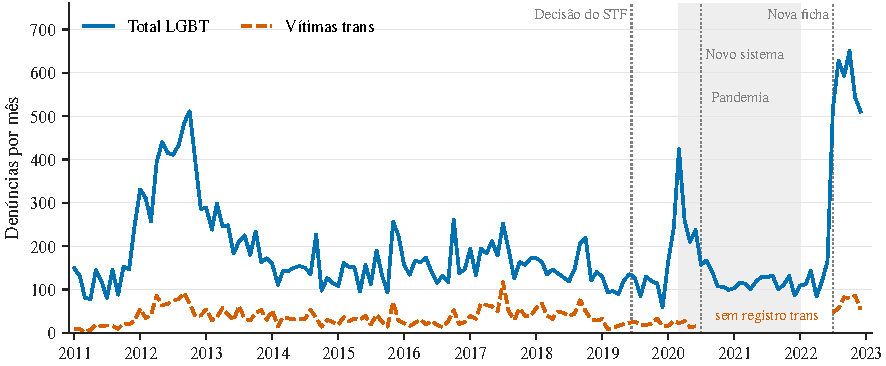
\includegraphics[width=\textwidth]{figuras/fig1_serie_mensal.pdf}
\caption{Denúncias mensais de violência contra pessoas LGBT (linha contínua azul) e contra vítimas trans (linha tracejada vermelha), 2011--2022. As linhas verticais pontilhadas marcam a decisão do STF e as mudanças no sistema de registro; a faixa cinza, a pandemia. Fonte: Disque 100 (ONDH/MDHC).}
\label{fig:serie}
\end{figure}

\subsection{Municípios com números alarmantes}

As denúncias se concentram em poucas cidades: as 10 com mais registros somam 28\% do total, e as 50 maiores, metade. Mas muitas denúncias não significam, por si só, alto risco: São Paulo tem o maior número absoluto, mas, proporcionalmente ao seu porte, fica apenas 31\% acima do esperado.

Depois de descontar o tamanho da população e o efeito do acaso nas cidades pequenas, \textbf{141 municípios tiveram números alarmantes em 2020--2022}. A maioria não é de grandes centros: 83 deles têm menos de 100 mil habitantes. Os casos mais extremos foram Ubaporanga (MG), com quase 30 vezes o esperado, Itaporanga (PB, 25 vezes), Cabo Frio (RJ, 17 vezes), Barbacena (MG, 10 vezes) e Campos dos Goytacazes (RJ, 8 vezes). Entre as capitais, destacam-se João Pessoa (3,4 vezes o esperado em 2011--2022) e Brasília (2,5 vezes).

Esses municípios não estão espalhados ao acaso. A análise de aglomerados identificou \textbf{61 municípios em regiões de alto risco}, concentrados na Zona da Mata e no Sul de Minas Gerais, na região metropolitana do Rio de Janeiro, no interior de São Paulo, em Goiás e no entorno de João Pessoa (Figura~\ref{fig:mapa}).

Também olhamos a tendência das 136 cidades com pelo menos 30 registros. Em 18 delas, as denúncias cresceram mais rápido que o total nacional, com destaque para Juazeiro (BA, +69\% ao ano), Itaporanga (PB, +68\%) e Barbacena (MG, +49\%), além de cidades do estado de São Paulo (Santos, Guarulhos, Sorocaba, Jundiaí) e da região metropolitana do Rio (Niterói, São Gonçalo). As capitais Rio de Janeiro, Belo Horizonte, Recife, São Paulo e Salvador também cresceram acima do total nacional, entre 5\% e 8\% ao ano. Em 15 cidades houve queda relativa, como Novo Hamburgo (RS), Rondonópolis (MT) e Teresina (PI).

\begin{figure}[H]
\centering
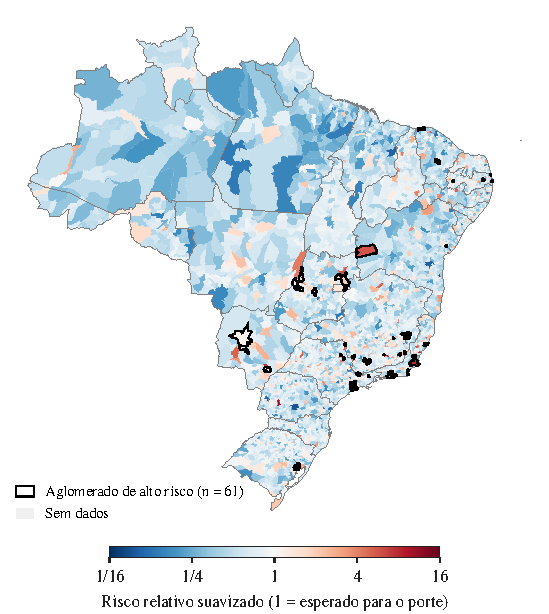
\includegraphics[width=0.62\textwidth]{figuras/fig3_mapa_risco.pdf}
\caption{Risco relativo suavizado de denúncias por município, 2020--2022. Vermelho: mais denúncias do que o esperado para o porte; azul: menos; branco: o esperado. O contorno preto marca os aglomerados de alto risco (Getis-Ord, $p<0{,}05$). Fonte: Disque 100 e IBGE.}
\label{fig:mapa}
\end{figure}

\subsection{O que explica e o que permite prever as ondas}

\textbf{É possível prever.} Os três modelos previram melhor do que distribuir as denúncias apenas pela população, enquanto as regras ingênuas foram piores (Tabela~\ref{tab:validacao} e Figura~\ref{fig:validacao}). O LightGBM teve o melhor resultado, com erro 16,7\% menor que a referência, seguido de perto pelo modelo endêmico-epidêmico (14,6\%). Repetir o número do ano anterior foi a pior estratégia: o número de denúncias de uma cidade varia muito de um ano para o outro, e o passado só ajuda quando combinado com as características do município.

O ganho mais importante está na antecipação de ondas. Das 20 cidades que o LightGBM apontou a cada ano como mais prováveis de ter uma onda, 37\% de fato a tiveram. Usando apenas a população, o acerto seria de 15\%. Ou seja, o modelo multiplica por 2,5 a capacidade de direcionar a atenção para as cidades certas.

\begin{table}[H]
\centering
\caption{Desempenho dos modelos na previsão um ano à frente (média de 2016 a 2022)}
\label{tab:validacao}
{\renewcommand{\arraystretch}{1.3}\small
\begin{tabular}{p{4.6cm} p{2.6cm} p{2.6cm} p{3.0cm}}
\hline
\textbf{Modelo} & \textbf{Redução do erro em relação à população} & \textbf{Acerto das 50 maiores cidades} & \textbf{Acerto entre as 20 cidades apontadas para onda} \\
\hline
LightGBM & 16,7\% & 66\% & 37\% \\
Endêmico-epidêmico & 14,6\% & 63\% & 31\% \\
Extra Trees & 11,3\% & 63\% & 31\% \\
Só população (referência) & -- & 63\% & 15\% \\
Fatia histórica da cidade & $-$14,7\% & 61\% & 29\% \\
Repetir o ano anterior & $-$35,8\% & 55\% & 26\% \\
\hline
\end{tabular}}
\end{table}

\begin{figure}[H]
\centering
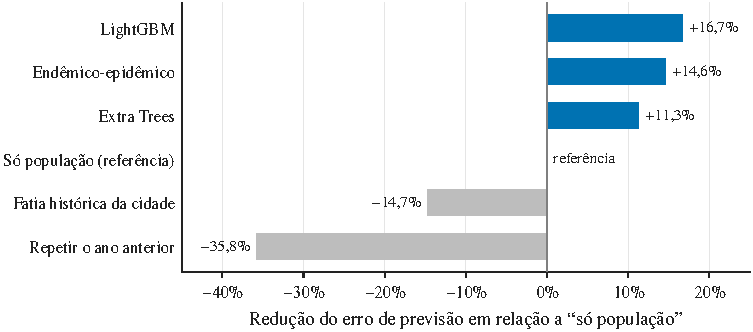
\includegraphics[width=0.85\textwidth]{figuras/fig2_validacao.pdf}
\caption{Redução do erro de previsão de cada modelo em relação à referência ``só população'' (média da validação de 2016 a 2022). Barras azuis: modelos de previsão; barras cinza: regras simples. Valores negativos indicam erro maior que o da referência. Fonte: Disque 100 e IBGE.}
\label{fig:validacao}
\end{figure}

\textbf{O que está associado a mais denúncias.} A Tabela~\ref{tab:coef} mostra as características dos municípios que se associam a mais ou menos denúncias do que o esperado para o seu porte. O fator mais forte foi a proporção de domicílios com casais do mesmo sexo, que é a melhor medida disponível do tamanho da população LGBT visível em cada cidade: municípios um pouco acima da média nesse indicador têm 12,5\% mais denúncias. A densidade demográfica teve efeito parecido (+12,4\%). A existência de uma ouvidoria municipal de direitos humanos esteve associada a 23\% mais denúncias, o que sugere que um canal institucional facilita a denúncia. Municípios com maior proporção de pretos e pardos denunciaram 8\% menos que o esperado. O Norte e o Sul denunciaram menos que o Sudeste, e o Centro-Oeste, mais. Renda, PIB, desigualdade, taxa de homicídios, índice de política LGBT e Processo Transexualizador não mostraram relação com o volume total de denúncias LGBT.

\begin{table}[H]
\centering
\caption{Características associadas a mais (RR $>$ 1) ou menos (RR $<$ 1) denúncias do que o esperado para o porte do município}
\label{tab:coef}
{\renewcommand{\arraystretch}{1.25}\small
\begin{tabular}{p{6.8cm} c c c}
\hline
\textbf{Característica} & \textbf{RR} & \textbf{IC 95\%} & \textbf{Há efeito?} \\
\hline
Casais do mesmo sexo (por desvio-padrão) & 1,13 & 1,08--1,18 & sim \\
Densidade demográfica (por desvio-padrão) & 1,12 & 1,07--1,18 & sim \\
População (por desvio-padrão) & 1,08 & 1,02--1,15 & sim \\
Pretos e pardos (por desvio-padrão) & 0,92 & 0,86--0,98 & sim \\
Tem ouvidoria de direitos humanos & 1,23 & 1,10--1,37 & sim \\
Região Centro-Oeste (em relação ao Sudeste) & 1,36 & 1,17--1,57 & sim \\
Região Sul & 0,72 & 0,64--0,81 & sim \\
Região Norte & 0,58 & 0,48--0,70 & sim \\
Renda domiciliar por pessoa & 1,01 & 0,92--1,10 & não \\
Taxa de homicídios no ano anterior & 0,99 & 0,94--1,03 & não \\
Índice de política LGBT (MUNIC) & 0,99 & 0,96--1,01 & não \\
Processo Transexualizador ativo & 0,71 & 0,34--1,46 & não \\
\hline
\multicolumn{4}{p{12cm}}{\footnotesize Modelo endêmico-epidêmico, 2012--2022. Também incluídos, sem efeito: PIB por pessoa, índice de Gini, população de 15 a 29 anos, estrutura municipal de direitos humanos, capital e região Nordeste.}
\end{tabular}}
\end{table}

\textbf{As ondas são locais.} O modelo endêmico-epidêmico permite separar a origem das denúncias esperadas. Em média, 74\% vêm das características do próprio município, 26\% da inércia (cidades com muitas denúncias num ano tendem a ter muitas no seguinte, sobretudo as grandes) e apenas 0,3\% das cidades vizinhas. Em outras palavras, as ondas observadas \textit{não se espalham} para os municípios do entorno: elas nascem e permanecem locais. O LightGBM chegou à mesma conclusão: as informações que mais pesaram nas suas previsões foram o histórico da própria cidade, a proporção de casais do mesmo sexo e a densidade demográfica.

\textbf{Alertas.} A cada ano, entre 22 e 52 municípios entraram em alerta. A maioria das ondas é passageira, mas uma cidade em alerta tem quase 6 vezes mais chance de voltar a ficar em alerta no ano seguinte do que uma cidade qualquer. Os alertas que se repetiram ao longo dos anos aparecem em cidades pequenas e médias de Minas Gerais (Cambuí, Ubaporanga, Caratinga, Muriaé), da Paraíba (Cajazeiras, Itaporanga), de Pernambuco (Ouricuri) e do Paraná (Guaraniaçu). Para 2023, supondo que o país registrasse o mesmo volume de 2022, as maiores chances de onda estimadas foram para Barbacena (MG, 40\%) e, com cerca de 30\%, Fortaleza, Cabo Frio, São Paulo, Campo Grande, Rio de Janeiro e Santos.

\subsection{Como o modelo aprende e por que confiar na previsão}

Um modelo de aprendizado de máquina só é útil se aprender padrões que se repetem, e não detalhes de um ano específico. Por isso, examinamos o LightGBM por quatro ângulos.

\textbf{Ele aprende, e sabe a hora de parar.} O LightGBM constrói árvores de decisão uma a uma, cada nova árvore corrigindo os erros das anteriores. A Figura~\ref{fig:curvas}a mostra esse processo no treino que prevê 2022. O erro nos dados de treino cai continuamente, mas o erro no ano reservado para conferência para de cair depois de cerca de 750 árvores. A partir daí, o modelo passaria a memorizar o passado em vez de aprender com ele. A Figura~\ref{fig:curvas}b mostra o mesmo nos sete anos previstos: o erro de conferência cai até um ponto mínimo (os círculos, onde o treino foi interrompido) e depois volta a subir em vários anos, até 11\% acima do mínimo. Essa interrupção automática é o que impede o sobreajuste.

\begin{figure}[H]
\centering
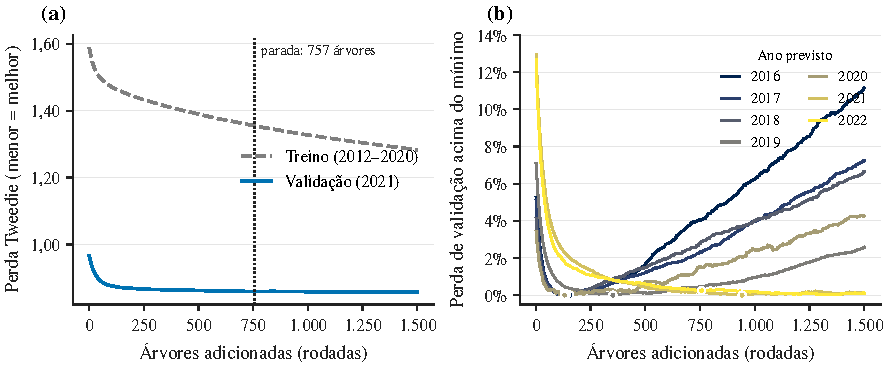
\includegraphics[width=\textwidth]{figuras/fig5_curvas_aprendizado.pdf}
\caption{Aprendizado do LightGBM ao longo das árvores. (a) Previsão de 2022: erro no treino (cinza tracejado) e no ano reservado para conferência (azul); a linha pontilhada marca onde o treino parou. (b) Erro de conferência acima do seu mínimo, para cada ano previsto; os círculos marcam o ponto de parada. Fonte: Disque 100 e IBGE.}
\label{fig:curvas}
\end{figure}

\textbf{O ganho é real, e não fruto do acaso.} Reamostrando os municípios 2.000 vezes (\textit{bootstrap}), a redução do erro do LightGBM em relação à referência populacional ficou entre 13,3\% e 20,3\% (intervalo de 95\%). Ele foi melhor que a referência em todos os sete anos testados e melhor que o modelo endêmico-epidêmico em seis deles. A vantagem sobre o endêmico-epidêmico é pequena, de 2,1 pontos percentuais (IC 95\%: 0,1 a 4,2), mas estatisticamente consistente. O resultado também não depende de ajuste fino: variando os principais parâmetros do algoritmo (número de folhas, taxa de aprendizado, tamanho mínimo das folhas, tipo de perda), o ganho médio por ano ficou sempre entre 15,7\% e 17,3\%.

\textbf{De onde vem o ganho.} Treinando o modelo com partes das informações, as características estruturais do município, sozinhas, já reduzem o erro em 14,0\%. O histórico da própria cidade, sozinho, também reduz 14,1\%. Juntos, chegam a 16,7\%. A informação sobre os municípios vizinhos acrescenta apenas 0,15 ponto, o que confirma, por outro caminho, que as ondas não se propagam entre cidades vizinhas.

\textbf{As previsões são calibradas e úteis para priorizar.} Agrupando as previsões em faixas, a média prevista acompanha a média observada desde os municípios com menos de 0,01 denúncia esperada por ano até os que têm mais de cinco (Figura~\ref{fig:calib}a). No total, o LightGBM previu 96\% das denúncias que de fato ocorreram. Para fins de vigilância, o que importa é a priorização (Figura~\ref{fig:calib}b): monitorando apenas 1\% dos municípios por ano (cerca de 56 cidades), os escolhidos pelo LightGBM concentram 31\% de todas as ondas de 2016 a 2022, contra 22\% se a escolha fosse pela população. Com 5\% dos municípios, a captura chega a 69\%. A vantagem do modelo está justamente no topo da lista, onde a atenção é mais escassa.

\begin{figure}[H]
\centering
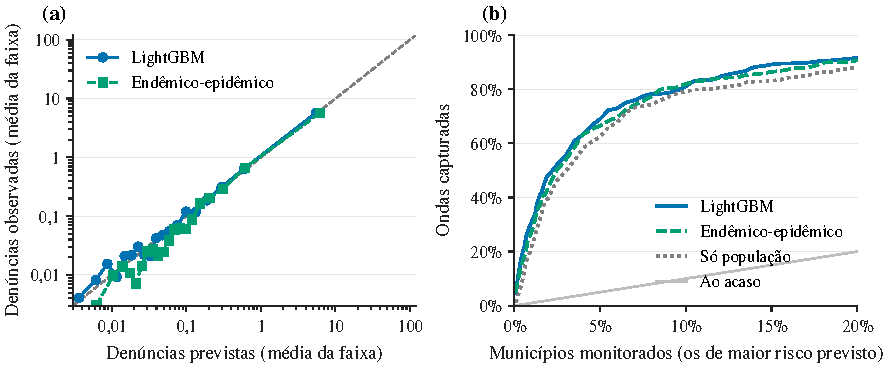
\includegraphics[width=\textwidth]{figuras/fig8_calibracao_captura.pdf}
\caption{(a) Calibração: denúncias previstas e observadas, por faixa de previsão (escala log); a linha tracejada indica previsão perfeita. (b) Percentual das 332 ondas de 2016 a 2022 capturado quando se monitoram os municípios de maior risco previsto; a linha cinza indica a escolha ao acaso. Previsões fora da amostra. Fonte: Disque 100 e IBGE.}
\label{fig:calib}
\end{figure}

\textbf{O que o modelo aprendeu.} Os valores SHAP mostram quanto cada informação empurrou cada previsão para cima ou para baixo (Figura~\ref{fig:shap}). O modelo aprendeu quatro regras principais, todas coerentes com a análise estatística: cidades com histórico de denúncias acima do esperado continuam acima; mais casais do mesmo sexo e maior densidade aumentam as denúncias esperadas, com efeito que se estabiliza a partir de níveis médios; e municípios com maior proporção de pretos e pardos têm menos denúncias que o esperado. Como o modelo de aprendizado de máquina, sem nenhuma hipótese prévia, chegou às mesmas relações do modelo estatístico, há mais confiança de que elas são padrões dos dados, e não artefatos de um método.

\begin{figure}[H]
\centering
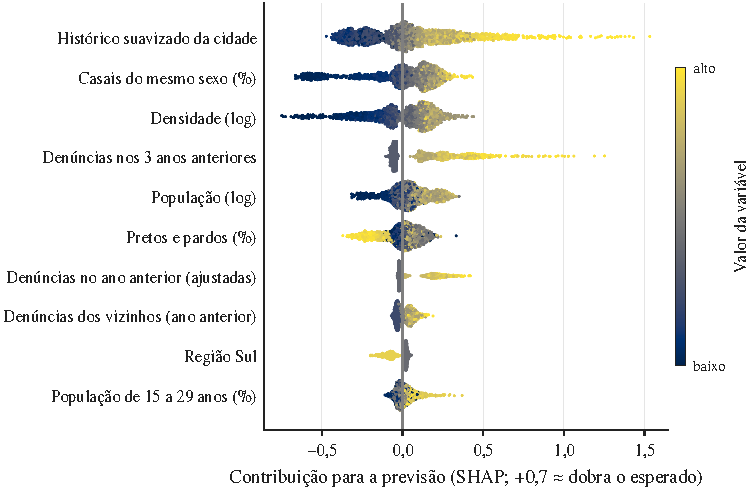
\includegraphics[width=0.85\textwidth]{figuras/fig9_shap_enxame.pdf}
\caption{Contribuição de cada informação para as previsões do LightGBM (valores SHAP, 4.000 municípios-ano). Cada ponto é um município num ano; a cor indica se o valor da variável é baixo (azul-escuro) ou alto (amarelo); pontos à direita do zero aumentam a previsão. As 10 variáveis mais importantes, em ordem. Fonte: Disque 100 e IBGE.}
\label{fig:shap}
\end{figure}

\subsection{Violência contra pessoas trans: proporção e perfil}

\textbf{Proporção.} Nos períodos em que a identidade de gênero podia ser registrada, 18\% das denúncias LGBT tinham vítima trans (4.406 de 24.151). Esse percentual oscilou muito de um ano para outro, entre 8\% e 31\%, acompanhando as mudanças no formulário. Comparando municípios dentro de um mesmo ano, a proporção de vítimas trans foi maior no Nordeste (chance 54\% maior que no Sudeste) e menor em cidades mais densas e com mais pretos e pardos. O Processo Transexualizador não teve relação com essa proporção. Nas capitais, cidades com mais políticas LGBT tiveram uma fatia trans \textit{menor}. Uma explicação possível é que essas políticas facilitam sobretudo a denúncia por outras vítimas LGBT, o que reduz o peso relativo das vítimas trans. Os municípios alarmantes não diferem dos demais nesse ponto (17\% contra 19\%): as ondas atingem a comunidade LGBT como um todo.

\textbf{Perfil.} A violência contra pessoas trans é mais grave e mais pública (Figura~\ref{fig:perfil}). Quando a denúncia envolve violação contra a vida, a chance de a vítima ser trans é 3 vezes maior. Também é maior na violência sexual (1,7 vez) e física (1,4 vez), e menor nas violências psicológica e de discriminação, mais comuns entre as demais vítimas LGBT. A violência contra pessoas trans acontece mais na rua e menos no trabalho, e é praticada mais por desconhecidos (1,7 vez), por profissionais ou agentes de instituições (2,3 vezes) e em relações de trabalho (1,9 vez). As vítimas trans são mais jovens, concentradas entre 25 e 29 anos.

Os registros de vítimas trans também são \textbf{mais incompletos}: a raça/cor falta em 30\% deles, contra 16\% nos demais, e a relação com o agressor falta em 41\%, contra 23\%. Essa lacuna dificulta entender como raça e identidade de gênero se combinam na violência. O modelo distingue os dois grupos de forma moderada (AUC de 0,71, numa escala em que 0,5 é acaso e 1 é perfeito), e o LightGBM não foi melhor que a regressão logística. Isso indica que cada característica pesa de forma independente, sem combinações complexas entre elas.

\begin{figure}[H]
\centering
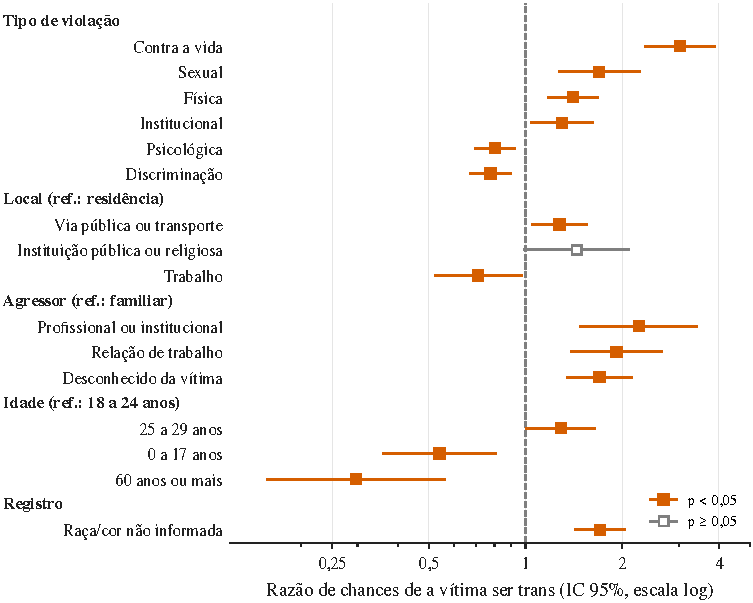
\includegraphics[width=0.85\textwidth]{figuras/fig4_perfil_trans.pdf}
\caption{Quanto cada característica da denúncia aumenta (à direita de 1) ou reduz (à esquerda de 1) a chance de a vítima ser trans. Quadrados cheios: efeito estatisticamente significativo ($p<0{,}05$); quadrados vazados em cinza: sem efeito. As linhas horizontais mostram o intervalo de confiança de 95\%. Fonte: Disque 100 (ONDH/MDHC).}
\label{fig:perfil}
\end{figure}

\subsection{Efeitos da Inclusão da Transfobia na Lei do Racismo}

O Supremo Tribunal Federal (STF) incluiu a transfobia (e a homofobia) nos crimes previstos na Lei do Racismo (Lei nº 7.716/1989) em 13 de junho de 2019.

\textbf{Total de denúncias LGBT.} Não houve mudança no nível de denúncias após a decisão (RR 0,98, IC 95\%: 0,67--1,43). Houve um crescimento leve nos meses seguintes, mas ele desaparece quando a análise se limita ao período antes das trocas de sistema (Tabela~\ref{tab:its}). As mudanças administrativas, ao contrário, tiveram efeitos enormes: a troca de sistema reduziu o volume em 59\%, e o novo formulário de 2022 o multiplicou por 4,5.

\textbf{Denúncias com vítima trans.} À primeira vista, as denúncias trans caíram 48\% após a decisão. O teste de placebo, porém, mostrou que essa queda começou em \textbf{fevereiro de 2019, quatro meses antes da decisão}. Ela coincide com uma mudança na forma de registrar: os casos marcados como ``travesti'' caíram de 32 no último trimestre de 2018 para 9 no primeiro trimestre de 2019. A queda, portanto, não é efeito da decisão, e sim de uma alteração no próprio registro.

\textbf{Conclusão desta análise.} Com os dados do Disque 100 não é possível medir o efeito da decisão do STF. Há apenas 13 meses de registros de vítimas trans depois dela, em parte sobrepostos ao início da pandemia, seguidos de dois anos sem essa informação. Esse resultado negativo também é um achado: ele mostra que as mudanças na forma de registrar as denúncias pesam mais nos números do que os marcos legais.

\begin{table}[H]
\centering
\caption{Mudança nas denúncias após a decisão do STF (13/06/2019)}
\label{tab:its}
{\renewcommand{\arraystretch}{1.25}\small
\begin{tabular}{p{4.4cm} p{3.4cm} p{4.6cm}}
\hline
\textbf{Série (período)} & \textbf{Mudança de nível (IC 95\%)} & \textbf{Leitura} \\
\hline
Total LGBT (2011--2022) & 0,98 (0,67--1,43) & sem mudança \\
Total LGBT (2011--jun/2020) & 0,84 (0,61--1,16) & sem mudança \\
Vítimas trans (2011--jun/2020) & 0,52 (0,33--0,80) & queda, mas iniciada em fev/2019 (placebo) \\
Proporção trans (2011--jun/2020) & 0,54 (0,38--0,75) & idem \\
\hline
\multicolumn{3}{p{12.4cm}}{\footnotesize Valores menores que 1 indicam queda. O modelo desconta tendência, sazonalidade, pandemia e mudanças de sistema.}
\end{tabular}}
\end{table}


\section{Conclusão}

Este trabalho mostrou que é possível localizar, entre os 5.565 municípios brasileiros, aqueles em que a violência contra pessoas LGBT é denunciada muito acima do esperado e antecipar onde tendem a surgir ondas de denúncias. Os números alarmantes não estão apenas nas capitais: dos 141 municípios alarmantes em 2020--2022, 83 têm menos de 100 mil habitantes, e eles se agrupam em regiões como a Zona da Mata e o Sul de Minas Gerais, o entorno do Rio de Janeiro e de João Pessoa. Na previsão de um ano à frente, o LightGBM foi o melhor modelo. Ele aprende de forma controlada, parando antes de memorizar o passado; seu ganho se mantém no \textit{bootstrap}, em todos os anos testados e com diferentes parâmetros; e ele chega às mesmas relações que o modelo estatístico. O resultado mais útil para a prática é a priorização: acompanhando só 1\% dos municípios, a lista do modelo reúne quase um terço das ondas. O modelo endêmico-epidêmico ficou pouco atrás e tem a vantagem de explicar a origem do risco. Por isso, os dois se complementam: um para ordenar as cidades, o outro para entender por que estão na lista.

\textbf{O que leva a mais denúncias.} Os fatores associados a mais registros indicam onde a denúncia acontece, e não necessariamente onde há mais violência. Denuncia-se mais onde a população LGBT é mais visível (mais casais do mesmo sexo), em cidades mais densas e onde a prefeitura mantém uma ouvidoria de direitos humanos, ou seja, onde existe um canal institucional próximo para receber a denúncia. Denuncia-se menos no Norte e no Sul e em municípios com maior proporção de pessoas pretas e pardas. Esses resultados são compatíveis com subnotificação nesses lugares, mas os dados não permitem separar menos violência de menos denúncia. Indicadores de riqueza, desigualdade e homicídios não explicaram o volume de denúncias, e as ondas não se espalharam para as cidades vizinhas: elas nascem e permanecem locais, e uma cidade em alerta tem quase seis vezes mais chance de voltar a ficar em alerta no ano seguinte. A maior parte das denúncias (70\% desde 2020) é feita pela própria vítima, quase sempre por telefone.

\textbf{A violência contra pessoas trans.} As vítimas trans são uma fração pequena das denúncias (18\%), mas sofrem uma violência diferente: mais grave (violações contra a vida, sexual e física), mais pública (na rua) e mais praticada por desconhecidos e por profissionais ou agentes de instituições. Esse último ponto importa para a pergunta sobre quem recebe a denúncia: quando o agressor está nas próprias instituições, denunciar por elas tende a ser mais difícil. A proporção de vítimas trans é maior no Nordeste e seus registros são os mais incompletos, com raça/cor e relação com o agressor faltando com muito mais frequência. As ondas de denúncias, por outro lado, atingem a comunidade LGBT como um todo, sem aumento da fatia trans nos municípios alarmantes. O Processo Transexualizador, presente em poucas cidades e com atividade em só dez delas no período, não mostrou relação com o número de denúncias nem com a proporção de vítimas trans.

\textbf{A decisão do STF.} Não foi possível afirmar que a inclusão da transfobia na Lei do Racismo, em 2019, alterou o número de denúncias. O total LGBT não mudou, e a queda nas denúncias trans começou quatro meses antes da decisão, junto com uma mudança na forma de registrar a categoria ``travesti''. Além disso, o Disque 100 deixou de registrar a identidade trans entre julho de 2020 e junho de 2022, o que deixa apenas 13 meses de observação após a decisão. As trocas de sistema e de formulário mudaram o volume nacional muito mais do que qualquer marco legal, o que é, por si só, um alerta para quem usa essas bases.

\textbf{Limitações.} O Disque 100 mede denúncias, e não a violência em si. Este é um estudo ecológico: as associações valem para municípios e não podem ser atribuídas a pessoas. A proporção de casais do mesmo sexo só existe no Censo de 2022, e a previsão trata o volume nacional do ano seguinte como conhecido, porque ele depende de decisões administrativas que os modelos não conseguem antecipar. Os dados terminam em 2022, de modo que as estimativas para 2023 ainda não foram conferidas.

\textbf{Trabalhos futuros e recomendações.} Três passos fortaleceriam os resultados: manter um campo estável de identidade de gênero no Disque 100, para que a série trans não tenha lacunas; cruzar as denúncias com o Sinan e o SIM, para comparar denúncia, atendimento e morte; e atualizar o painel com os dados de 2023 em diante, para testar a previsão em anos novos. Na gestão pública, a lista de municípios prioritários do modelo pode orientar onde reforçar canais de denúncia e acolhimento, a começar pela criação de ouvidorias nas cidades com risco alto e pouca estrutura.

\appendix

\section{Fórmulas e dicionário de variáveis}

Este apêndice reúne as fórmulas citadas no Método. A Tabela~\ref{tab:dicionario}, ao final, explica cada símbolo.

\subsection*{A1. Valor esperado de denúncias}
Número de denúncias que o município $i$ teria no ano $t$ se recebesse uma fatia do total nacional proporcional à sua população:
\begin{equation*}
E_{it} = N_t \times \frac{P_{it}}{\sum_j P_{jt}}
\end{equation*}

\subsection*{A2. Risco relativo suavizado (Bayes empírico Poisson-Gama)}
O risco relativo bruto é $y_i/E_i$. A versão suavizada aproxima os municípios pequenos da média nacional:
\begin{equation*}
\widehat{RR}_i = \frac{y_i + \alpha}{E_i + \beta}, \qquad
P(RR_i > 1) = 1 - F_{\text{Gama}}\!\left(1;\; y_i+\alpha,\; E_i+\beta\right)
\end{equation*}
em que $\alpha$ e $\beta$ são estimados a partir de todos os municípios pelo método dos momentos \cite{marshall:1991}. O município é alarmante quando $P(RR_i>1) > 0{,}95$.

\subsection*{A3. Estatística local de Getis-Ord}
\begin{equation*}
G_i^{*} = \frac{\sum_{j} w_{ij}\, \widehat{RR}_j - \bar{R}\sum_j w_{ij}}{s\sqrt{\left[n\sum_j w_{ij}^2 - \left(\sum_j w_{ij}\right)^2\right]/(n-1)}}
\end{equation*}
em que $w_{ij}=1$ se $j$ é o próprio município ou um dos seus 10 vizinhos mais próximos, e 0 caso contrário; $\bar{R}$ e $s$ são a média e o desvio-padrão do risco relativo no país. A significância foi obtida por 999 permutações. Aglomerado alto: $G_i^{*}>0$, $p<0{,}05$ e $\widehat{RR}_i>1$.

\subsection*{A4. Modelo endêmico-epidêmico Binomial Negativo}
\begin{equation*}
y_{it} \sim \text{BN}(\mu_{it}, \theta), \qquad
\mu_{it} = \underbrace{e^{\mathbf{x}_{it}^{\top}\boldsymbol{\beta}}\, E_{it}}_{\text{estrutural}}
+ \underbrace{\lambda_i\, r_t\, y_{i,t-1}}_{\text{inércia}}
+ \underbrace{\phi_i\, r_t\, \bar{y}_{\mathcal{V}(i),t-1}}_{\text{vizinhança}}
\end{equation*}
\begin{equation*}
r_t = \frac{N_t}{N_{t-1}}, \qquad \log\lambda_i = a_0 + a_1 z_i, \qquad \log\phi_i = c_0 + c_1 z_i
\end{equation*}
em que $z_i$ é o log da população padronizado. Parâmetros estimados por máxima verossimilhança \cite{held_hohle_hofmann:2005}. Para o LightGBM e o Extra Trees, $\log E_{it}$ entra como termo fixo (\textit{offset}) ou como variável, e o LightGBM usa perda Tweedie com potência 1,3.

\textit{Métricas de validação.} Desvio de Poisson médio: $D = \frac{2}{n}\sum_i \left[y_i \log(y_i/\hat{\mu}_i) - (y_i-\hat{\mu}_i)\right]$. Redução do erro: $1 - D_{\text{modelo}}/D_{\text{só população}}$.

\subsection*{A5. Onda e alerta}
\begin{equation*}
\text{onda}_{it} = 1 \;\text{ se }\; y_{it} \ge 5 \;\text{ e }\; y_{it} \ge 2E_{it}; \qquad
\text{alerta}_{it} = 1 \;\text{ se }\; y_{it} > q_{0,95}(\hat{\mu}_{it}, \hat{\theta}) \;\text{ e }\; y_{it} \ge 3
\end{equation*}
em que $q_{0,95}$ é o percentil 95 da distribuição Binomial Negativa prevista pelo modelo A4 (alerta forte: percentil 99).

\subsection*{A6. Regressão binomial da proporção de vítimas trans}
\begin{equation*}
\text{logit}\!\left(\pi_{it}\right) = \gamma_t + \mathbf{x}_{it}^{\top}\boldsymbol{\beta}, \qquad
y^{\text{trans}}_{it} \sim \text{Binomial}(n_{it}, \pi_{it})
\end{equation*}
em que $n_{it}$ é o número de denúncias LGBT feitas em períodos com registro de identidade trans e $\gamma_t$ é o efeito de cada ano. A sobredispersão foi estimada (quase-binomial), com erros-padrão agrupados por município.

\subsection*{A7. Regressão logística do perfil da vítima}
\begin{equation*}
\text{logit}\, P(\text{vítima trans}_k = 1) = \gamma_{t(k)} + \mathbf{v}_k^{\top}\boldsymbol{\beta}
\end{equation*}
em que $\mathbf{v}_k$ reúne as características da denúncia $k$: tipos de violação, local, relação com o agressor, faixa etária, raça/cor e região. Razão de chances $=e^{\beta}$. Erros-padrão agrupados por município. Comparação com o LightGBM por validação cruzada agrupada por município (5 partições, AUC).

\subsection*{A8. Série temporal interrompida}
\begin{multline*}
\log \mathrm{E}[Y_m] = \beta_0 + \beta_1 m + \beta_2\, D_m + \beta_3 (m-m_0)\, D_m + \boldsymbol{\gamma}^{\top}\mathbf{c}_m \\
+ \sum_{k=1}^{2}\left[\delta_k \sin\tfrac{2\pi k\, \text{mês}}{12} + \eta_k \cos\tfrac{2\pi k\, \text{mês}}{12}\right]
\end{multline*}
em que $D_m=1$ a partir de junho de 2019; $e^{\beta_2}$ é a mudança de nível e $e^{\beta_3}$ a mudança de tendência mensal. Binomial Negativa para contagens e binomial para a proporção trans, com erros de Newey-West (6 defasagens) \cite{bernal:2017}. No teste de placebo, $m_0$ percorre todos os meses de 2018 e 2019, e o melhor ponto de quebra é o de maior log-verossimilhança.

\begin{table}[H]
\centering
\caption{Dicionário de símbolos}
\label{tab:dicionario}
{\renewcommand{\arraystretch}{1.2}\small
\begin{tabular}{p{2.6cm} p{10.6cm}}
\hline
\textbf{Símbolo} & \textbf{Significado} \\
\hline
$i$, $j$; $t$; $m$; $k$ & município; ano; mês; denúncia \\
$y_{it}$ & denúncias LGBT observadas no município $i$, ano $t$ \\
$N_t$ & total nacional de denúncias LGBT no ano $t$ \\
$P_{it}$ & população do município \\
$E_{it}$ & denúncias esperadas pelo porte (A1) \\
$RR_i$, $\widehat{RR}_i$ & risco relativo (observado/esperado) bruto e suavizado \\
$\alpha$, $\beta$ & parâmetros da distribuição Gama usada na suavização \\
$w_{ij}$; $\mathcal{V}(i)$ & peso de vizinhança; conjunto dos 10 vizinhos mais próximos de $i$ \\
$\mu_{it}$; $\theta$ & número esperado de denúncias segundo o modelo; parâmetro de dispersão da Binomial Negativa \\
$\mathbf{x}_{it}$ & características do município: população, densidade, renda, PIB e homicídios do ano anterior, Gini, \% de 15 a 29 anos, \% de pretos e pardos, \% de casais do mesmo sexo, índice LGBT da MUNIC, ouvidoria, estrutura de direitos humanos, Processo Transexualizador, capital e região \\
$\boldsymbol{\beta}$ & efeitos das características; $e^{\beta}$ é a razão de taxas (RR) ou de chances \\
$\lambda_i$; $\phi_i$ & intensidade da inércia; intensidade da propagação entre vizinhos \\
$r_t$ & razão entre o total nacional do ano e o do ano anterior \\
$\pi_{it}$; $n_{it}$ & proporção de vítimas trans; denúncias LGBT no período com registro de identidade trans \\
$\gamma_t$ & efeito fixo do ano \\
$D_m$; $m_0$ & indicador de período após a decisão do STF; mês da decisão (ou do placebo) \\
$\mathbf{c}_m$ & controles: pandemia (mar/2020--dez/2021), novo sistema (a partir de jul/2020) e nova ficha (a partir de jul/2022) \\
DP & desvio-padrão: as variáveis contínuas foram padronizadas para média 0 e DP 1 \\
IC 95\% & intervalo de confiança de 95\% \\
AUC & área sob a curva ROC: 0,5 equivale ao acaso e 1 à classificação perfeita \\
\hline
\end{tabular}}
\end{table}


\bibliographystyle{sbc}
\bibliography{sbc-template,referencias_metodo}

\end{document}
